%!TEX root = paper.tex
\usetikzlibrary{shapes.misc, positioning}
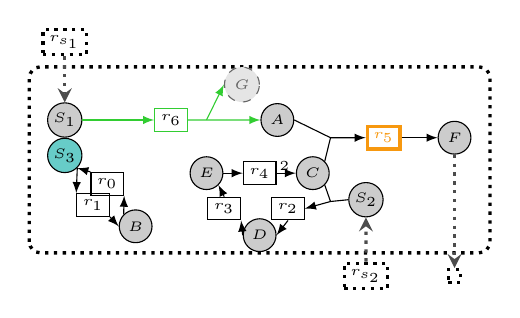
\begin{tikzpicture}[scale=0.45]\tiny
  \tikzstyle{metabolite}=[draw,circle,fill=white!80!black, text width=0.4cm, inner sep=0pt, align=center];
  \tikzstyle{repairmetabolite}=[draw,white!40!black, circle,fill=white!90!black,text=white!40!black,dashed];
  \tikzstyle{seed}=[draw,circle,fill=BlueGreen!70, text width=0.4cm, inner sep=0pt, align=center];%white!80!black
  \tikzstyle{target}=[draw,circle,fill=YellowOrange];%white!40!black
  \tikzstyle{reaction}=[draw,rectangle];
   \tikzstyle{export}=[draw,rectangle,dotted, very thick];
   \tikzstyle{exportrepair}=[draw,rectangle,dotted, very thick,white!80!black,text=white!70!black];
  \tikzstyle{repairreaction}=[draw,rectangle,white!40!black,text=white!40!black,dashed];
  \tikzstyle{solreaction}=[draw,rectangle,LimeGreen,text=black];
  \tikzstyle{initial}=[->,>=latex,thick];
  \tikzstyle{bdd}=[->,>=latex,thick];
  \tikzstyle{etiq}=[midway,fill=black!20,scale=0.5];
  \tikzstyle{stc}=[draw, rectangle, white, text=black]

  \node[stc] (stcr4C) at (6.2,6.7) {$2$};

  \draw [black,dotted, rounded corners, very thick] (-1,4.25) rectangle (12,9.5);
 % \node (system) [draw, rounded rectangle] at (0,0) {} (7cm,5cm);

  \node[seed] (S2) at (0,7) {$S_{3}$};
  \node[metabolite] (Sb2) at (8.5,5.75) {$S_{2}$};
  \node[metabolite] (S1) at (0,8) {$S_{1}$};

  \node[metabolite] (F) at (11,7.50) {$F$};

  \node[metabolite] (A) at (6,8) {$A$};
  \node[metabolite] (B) at (2,5.0) {$B$};
  \node[metabolite] (C) at (7,6.5) {$C$};
  \node[metabolite] (D) at (5.50,4.75) {$D$};
  \node[metabolite] (E) at (4,6.5) {$E$};
  \node[repairmetabolite] (X) at (5,9) {$G$};

  \node[reaction] (R0) at (1.2,6.2) {$r_{0}$};
  \node[reaction] (R1) at (0.8,5.60) {$r_{1}$};
  \node[reaction] (R2) at (6.3,5.5) {$r_{2}$};
  \node[reaction] (R3) at (4.5,5.5) {$r_{3}$};
  \node[reaction] (R4) at (5.5,6.5) {$r_{4}$};
  \node[reaction, very thick,YellowOrange] (R5) at (9,7.50) {$r_{5}$}; %LimeGreen
  \node[solreaction] (R6) at (3,8) {$r_{6}$};
  % \node[repairreaction] (R7) at (2.3,6.9) {$r_{7}$};
  % \node[repairreaction] (R8) at (3,5.8) {$r_{8}$};
  % \node[repairreaction] (R9) at (8.5,8.5) {$r_{9}$};

  % R0 : S => B
  \draw[->,>=latex] (B.north west) -- (R0.south east);
  \draw[->,>=latex] (R0.north west) -- (S2.south east);

  % R1 : S <= B
  \draw[->,>=latex] (S2.south east) -- (R1.north west);
  \draw[->,>=latex] (R1.south east) -- (B.west);

  % R2 : Sb2+C => D
  \draw[->,>=latex] (Sb2.west) -- (7.5,5.70) -- (R2.east);
  \draw[] (C.south east) -- (7.5,5.70);
  \draw[->,>=latex] (R2.south) -- (D.east);

  % R3 : D => E
  \draw[->,>=latex] (D.west) -- (R3.south east);
  \draw[->,>=latex] (R3.north) -- (E.south east);

  % R4 : E => C
  \draw[->,>=latex] (E.east) -- (R4.west);
  \draw[->,>=latex] (R4.east) -- (C.west);

  % R5 : A+C => T
  \draw[->,>=latex] (A.east) -- (7.5,7.50) -- (R5.west);
  \draw[] (C.north east) -- (7.5,7.50);
  \draw[->,>=latex] (R5.east) -- (F.west);

  % R6 : S => A+X
  \draw[->,>=latex,LimeGreen] (S1.east) -- (R6.west);
  \draw[->,>=latex,LimeGreen] (R6.east) -- (4,8) -- (A.west);
  \draw[->,>=latex,LimeGreen] (4,8) -- (X.west);

  % % R7 : S => E
  % \draw[->,>=latex,white!55!black,dashed] (S2.east) -- (R7.west);
  % \draw[->,>=latex,white!55!black,dashed] (R7.east) -- (E.north west);
  %
  % % R8 : B => E
  % \draw[->,>=latex,white!55!black,dashed] (B.north east) -- (R8.south west);
  % \draw[->,>=latex,white!55!black,dashed] (R8.east) -- (E.south);

  % % R9 : X => F
  % \draw[->,>=latex,green] (X.east) -- (R9.north west);
  % \draw[->,>=latex,green] (R9.east) -- (F.north west);

  %export X
  %\node[exportrepair] (outX) at (6.5,10.30) {$r_{expX}$};
  %\draw[->,>=stealth,white!80!black,dotted, very thick] (X.north east) --  (outX.west);

  %export F
  \node[export] (outF) at (11,3.6) {\ExportReaction};
   \draw[->,>=stealth,white!30!black,dotted, very thick] (F.south) --  (outF.north);

  %import S2
   \node[export] (inS) at (0,10.2) {$r_{s_1}$};
   \draw[->,>=stealth,white!30!black,dotted, very thick] (inS.south) --  (S1.north);

   %import Sb2
  \node[export] (inS2) at (8.5,3.6) {$r_{s_2}$};
  \draw[->,>=stealth,white!30!black,dotted, very thick] (inS2) --  (Sb2.south);

\end{tikzpicture}
%
%%% Local Variables:
%%% mode: latex
%%% TeX-master: "paper"
%%% End:
